\uuid{7kQc}
\exo7id{4992}
\titre{exo7 4992}
\auteur{quercia}
\organisation{exo7}
\datecreate{2010-03-17}
\isIndication{false}
\isCorrection{true}
\chapitre{Courbes planes}
\sousChapitre{Courbes paramétrées}

\contenu{
\texte{
Déterminer les points doubles de la courbe d'équation polaire
$\rho = \frac{\theta}{\theta^2-1}$.
}
\reponse{
$$
\centerline{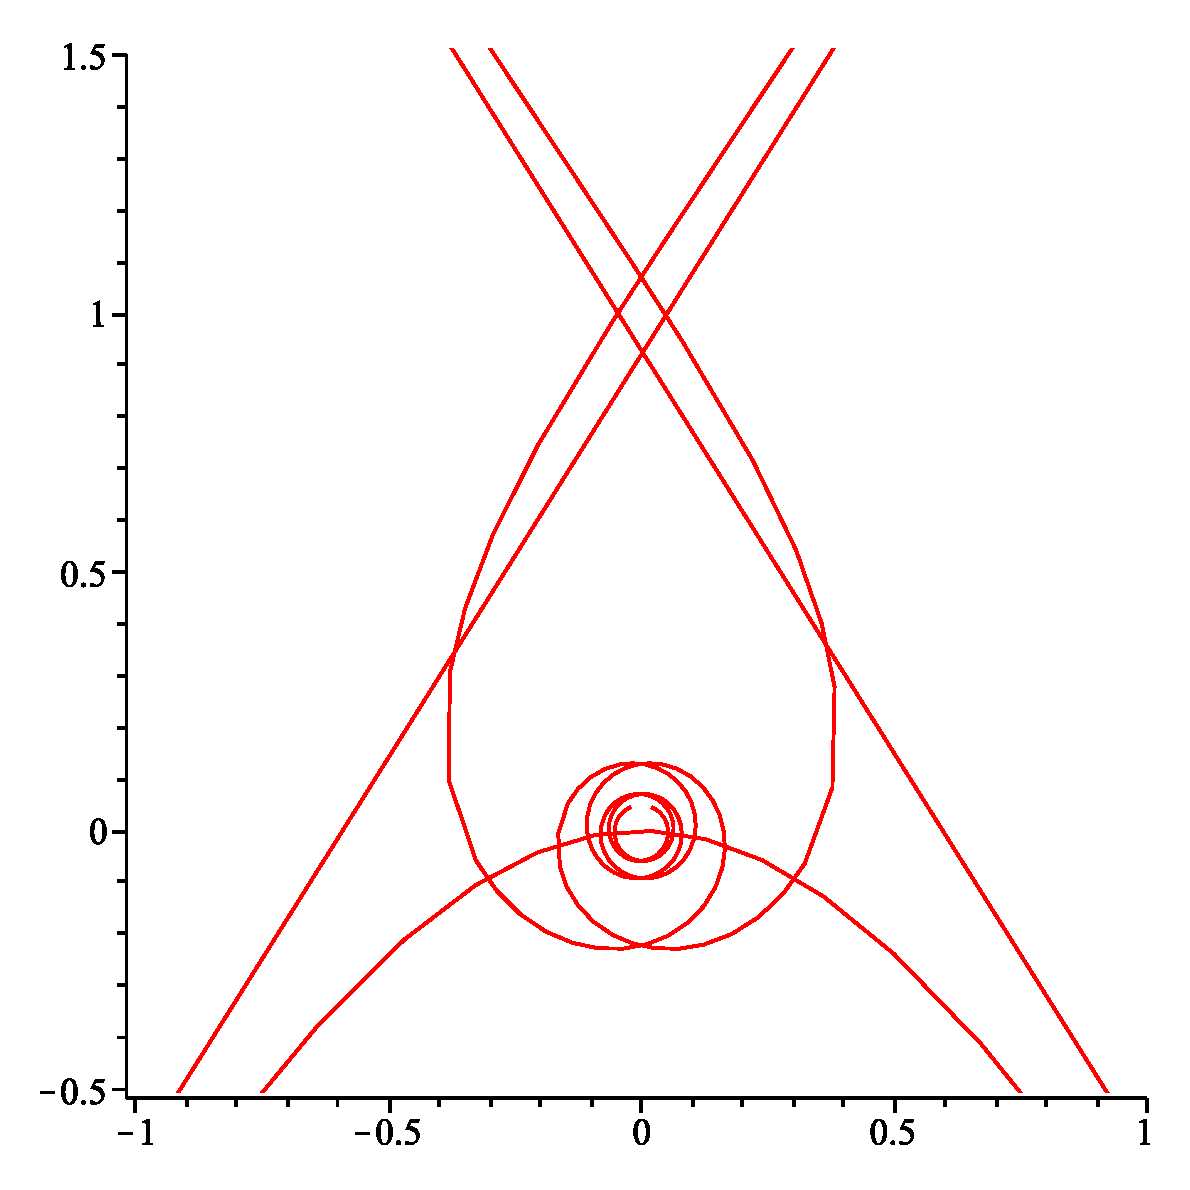
\includegraphics[height=4cm]{../images/img004992-1}}
$$
%\mapleplot{plot([t/(t^2-1),t,t=-20..20],x=-1..1,y=-0.5..1.5,coords=polar,axes=frame);}%

La courbe est symétrique par rapport à $Oy$. $M(\rho,\theta) = M_1(\rho_1,\theta_1)$
si et seulement si $\begin{cases}\theta_1\equiv \theta\ [2\pi]\cr \rho_1 = \rho\cr\end{cases}$
ou $\begin{cases}\theta_1\equiv \theta+\pi\ [2\pi]\cr \rho_1 = -\rho.\cr\end{cases}$

Dans le premier cas, $\rho=\rho_1 \Leftrightarrow \theta\theta_1 = -1$ pour
$\theta \ne \theta_1$ ce qui donne l'équation en $\theta$ :
$$\theta^2+2k\pi\theta+1 = 0$$
avec $k\in \Z$.
Cette équation à $k$ fixé non nul admet deux racines, ce qui donne deux
familles de points doubles.
De même, le second cas ammène deux autres familles définies par l'équation :
$$\theta^2+(2k+1)\pi\theta+1 = 0.$$
}
}
